\documentclass[final,3p,12pt,times,onecolumn,authoryear]{report}
\usepackage[brazil]{babel}
%\usepackage{tex4ht}
\usepackage{amssymb}
\usepackage{titling}
\usepackage[T1]{fontenc}
\usepackage{geometry}
\usepackage{url}
\usepackage{float}
\usepackage{caption}
\usepackage{amsthm,amsmath,mathtools,amssymb}
\usepackage{framed} 
\usepackage{multirow}
\usepackage{epstopdf}
\usepackage{multicol} 
\usepackage{varwidth}
\usepackage{color}
\usepackage{animate}
\usepackage{xcolor}
\usepackage{lmodern}
\usepackage{tikz}
\renewcommand*\familydefault{\sfdefault}
\usepackage{subfigure}
\usepackage{nomencl} 
\geometry{a4paper,left=2cm,right=2cm,bottom=2cm,top=2.5cm}
\setlength{\nomitemsep}{-\parskip}
\renewcommand{\baselinestretch}{0.9}
\renewcommand*\nompreamble{\begin{multicols}{2}}
\renewcommand*\nompostamble{\end{multicols}}
\usepackage[none]{hyphenat} 
 \usepackage{nomencl}
 \makenomenclature
\usepackage{lineno}
\usepackage{booktabs}
\usepackage{multirow}
\usepackage{pdfpages}
\usepackage{listings}
\lstset{
  language=C,                % choose the language of the code
  numbers=left,                   % where to put the line-numbers
  stepnumber=1,                   % the step between two line-numbers.        
  numbersep=5pt,                  % how far the line-numbers are from the code
  backgroundcolor=\color{white},  % choose the background color. You must add \usepackage{color}
  showspaces=false,               % show spaces adding particular underscores
  showstringspaces=false,         % underline spaces within strings
  showtabs=false,                 % show tabs within strings adding particular underscores
  tabsize=2,                      % sets default tabsize to 2 spaces
  captionpos=b,                   % sets the caption-position to bottom
  breaklines=true,                % sets automatic line breaking
  breakatwhitespace=true,         % sets if automatic breaks should only happen at whitespace
  title=\lstname,                 % show the filename of files included with \lstinputlisting;
  basicstyle=\footnotesize\ttfamily,
  keywordstyle=\bfseries\color{green!40!black},
  commentstyle=\itshape\color{purple!40!black},
  identifierstyle=\color{blue},
  stringstyle=\color{orange},
  }
  
% \lstdefinestyle{customc}{
%   belowcaptionskip=1\baselineskip,
%   breaklines=true,
%   frame=L,
%   xleftmargin=\parindent,
%   language=C,
%   showstringspaces=false,
%   basicstyle=\footnotesize\ttfamily,
%   keywordstyle=\bfseries\color{green!40!black},
%   commentstyle=\itshape\color{purple!40!black},
%   identifierstyle=\color{blue},
%   stringstyle=\color{orange},
% }

% \usepackage{minted}
%\journal{Applied Numerical Mathematics}
\newcommand{\red}[1]{\textcolor{red}{#1}}
\newcommand{\blue}[1]{\textcolor{blue}{#1}}
\pretolerance=1000 % for no overfull lines
\usepackage[
colorlinks=true,
pdfstartview=FitV,
linkcolor=blue,
citecolor=blue,
urlcolor=blue]{hyperref}
%\hypersetup{
   %pdftitle    ={Numerical modeling of chickpea \textit{(Cicer arietinum)} hydration: The effects of temperature and pressure},
   %pdfauthor   ={Pétterson Pramiu},
   %pdfkeywords = {diffusion equation \sep Fick's second law \sep the hydration process.},
	 %pdfsubject  = {Article}
%} 
 
\setlength{\parskip}{1em}
\linespread{1.25}
\hyphenation{especificamen-te} 

\begin{document}
\title{Relatório de estudos individual}
\author{Pétterson Vinícius Pramiu}
\date{\today}

\maketitle

\tableofcontents

\chapter{Introdução}
Este relatório objetiva registrar de forma detalhada e sistemática as atividades de pesquisa e estudos relacionados à temática de proposta de tese do autor. Nele serão revistos alguns conceitos fundamentais de mecânica de fluidos, métodos numéricos em equações diferenciais, instalação e configuração de bibliotecas para implementação computacional como PETSc e MPI, entre outros. Exemplos da resolução de sistemas de equações lineares e da solução de algumas EDPs como a equação de Laplace, de Poisson, da equação do calor transiente e da equação de Stokes serão resolvidos detalhadamente em diferenças finitas ou volumes finitos, empregando malhas estruturadas e em programação serial ou paralela. A linguagem selecionada para implementação dos códgidos fonte é a linguagem C, e alguns exemplos também serão ilustrados e implementados em Scilab. Com a realização destes exemplos espera-se obter os requisitos necessários para compreensão de trabalhos e implementação de código computacional envolvendo simulações em escoamentos turbulentos empregando o método de Simulação de Grandes Escalas - \textit{Large Eddy Simulation}.

\section{Motiva��o}

Dentre as ferramentas e abordagens amplamente utilizadas na engenharia contempor�nea em pesquisa e desenvolvimento de obras, m�quinas e processos, destacam-se aquelas associadas �s simula��es num�rico-computacionais, que decorrem do vertiginoso desenvolvimento de tecnologias da computa��o e de m�todos num�ricos sofisticados. Uma simula��o num�rico-computacional pode ser definida como aquela resultante da implementa��o em linguagem de programa��o de modelos matem�ticos e formula��es num�ricas que representa fen�menos ou eventos de interesse. S�o, geralmente, solu��es de sistemas de equa��es diferenciais, sistemas de equa��es estoc�sticas ou de equa��es alg�bricas, entre outros. Com custo relativo inferior � realiza��o de experimentos reais ou de modelos em escala, tais simula��es viabilizam o estudo de diversas combina��es de condi��es de utiliza��o, de modo a auxiliar na especifica��o de melhorias no projeto, opera��o e manuten��o de equipamentos, estruturas e processos.

Atualmente existem diversas ferramentas computacionais e softwares desenvolvidos especificamente para realiza��o de simula��es num�rico-computacionais. Softwares ou plataformas como o Ansys, Comsol, OpenFoam, MultiSim, Proteus, DualSPHyics, entre outros, s�o exemplos de tais ferramentas que s�o bem sucedidas nos seus campos, sendo amplamente utilizadas na engenharia. Esses softwares, em s�ntese, implementam modelos e formula��es que representam desde o comportamento de determinadas estruturas, o escoamento de fluidos, as trocas de calor, as correntes em circuitos el�tricos, entre outros. Al�m disso, em alguns deles a exemplo do Ansys, OpenFoam e DualSPHysics, � poss�vel a implementa��o explicita de modelos que n�o estejam previamente disponibilizados, por meio linguagens de programa��o pr�prias ou de outras usuais como C/C++, Fortran e XML.
	
Uma vasta �rea das Ci�ncias Aplicadas que emprega simula��o � a Din�mica de Fluidos Computacional, CFD, que trata de processos e fen�menos que apresentam escoamento. As aplica��es incluem o c�lculo das for�as e momentos em aeronaves, a determina��o da taxa de fluxo de massa de petr�leo em gasodutos, a previs�o de condi��es meteorol�gicas, a modelagem de detona��o de armas nucleares, o escoamento de fluidos em canais e abertos ou condutos for�ados. Para muitas delas, um resultado importante das simula��es envolvem a transfer�ncia de energia, press�o ou velocidade para estruturas que est�o em contato com o fluido. Esta an�lise viabiliza a quantifica��o dos esfor�os solicitados pelo escoamento.

Al�m das equa��es do momentum, algumas aplica��es que envolvem o transporte de quantidades requerem equa��es espec�ficas para modelar e resolver tal transporte. Exemplos s�o as equa��es para a energia, momento, tens�es, fluxos e outras quantidades envolvidas no escoamento. Outras quantidades tamb�m podem ser transportadas pelo fluido, mesmo que n�o estejam totalmente dispersas no fluido, a exemplo de part�culas suspensas ou arrastadas pelo escoamento. Esse caso, e v�rios outros usuais nas Engenharias, requerem modelos espec�ficos para a avalia��o do transporte das part�culas no meio fluido ou gasoso, sendo ent�o necess�ria a modelagem de diferentes fases, incluindo a fase particulada. Os modelos matem�ticos presentes em tais situa��es prov�m formula��o �s diferentes for�as de intera��o fluido-part�cula e para o c�lculo das trajet�rias das part�culas no meio cont�nuo ou fluido circundante.
	
A metodologia da CFD e essas concep��es podem ser empregadas para contribuir � formula��o e desenvolvimento de acuradas simula��es � avalia��o e predi��o do desgaste abrasivo-erosivo da superf�cie de materiais. Tal situa��o � especificamente importante � Usina Hidroel�trica de Itaipu, cuja superf�cie das lajes de concreto do vertedouro apresenta certo desgaste superficial decorrente dos mais de 30 anos de opera��o, requerendo interven��es e manuten��es curativas. Dada a atual impossibilidade de predizer matematicamente a evolu��o espa�o-temporal dos danos na referida estrutura, a CFD pode contribuir a tal an�lise. �, pois, relevante empreg�-la para investigar o efeito de distintos mecanismos de desgaste, sobretudo aqueles causados por escoamentos de �gua com e sem meio particulado.

Nesse tipo de estudo al�m dos modelos hidrodin�mico, de transporte e de part�culas, � indispens�vel � formula��o e o emprego de modelagem constitutiva para o material que comp�e a estrutura das calhas. Desafortunadamente a complexa natureza do concreto, resultante da sua heterogeneidade, da resposta assim�trica � tra��o e � compress�o, das mudan�as nas propriedades mec�nicas devidas � evolu��o da microfissura��o, do efeito de escala, entre outros fatores, t�m dificultado a formula��o de um modelo constitutivo geral e completo para o concreto.

Conhecidos ou calculados os for�antes, as solicita��es geradas pelo fluido ou part�culas transportadas s�o inseridas no modelo constitutivo do material, que viabiliza avaliar estados de tens�es da estrutura podendo, assim, indicar regi�es suscet�veis � ruptura e outros aspectos importantes na concep��o do projeto e opera��o da estrutura. Atualmente um dos modelos constitutivos promissores � modelagem do concreto � o Riedel-Hiermaier-Thoma, RHT, que representa o comportamento de materiais fr�geis de acordo com crit�rios de falha superficial.

Modelagens via CFD requerem as equa��es de Navier-Stokes completas, isto �, as equa��es da continuidade, momentum e transporte. Indispens�vel nessa abordagem �, ent�o, conhecer e resolver a turbul�ncia, que pode ser caracterizada pela mistura n�o linear e ca�tica das part�culas e elementos fluidos. Mais especificamente, um campo de fluxo turbulento � caracterizado por flutua��es de velocidade em todas as dire��es e escalas. 
%� invi�vel computacionalmente resolver diretamente as equa��es completas para problemas de porte muito menor que a da calha.

Processos de transporte de subst�ncias num dado ambiente podem ser grandemente acelerados pela presen�a de turbul�ncia. Com efeito, se considerada apenas o processo difusivo molecular, a propaga��o de certo material poderia demorar dias para se completar. Mas as for�as empuxo ou as correntes de escoamentos for�antes aceleram este processo para minutos, sobretudo devido a a��o da turbul�ncia. Assim, dada a relev�ncia da sua modelagem, existem diversas formula��es para sua representa��o, destacando-se � guisa de informa��o o modelo de zero equa��es, o modelo $k-\epsilon$, o modelo $k-\omega$, o modelo SST (Shear Stress Transpor), a modelagem RANS (Reynolds Avarage Navier Stokes) e a modelagem TLES (Temporal Large Eddy Scale).

Estudos e resultados preliminares obtidos em Projeto j� finalizado no CEASB/PTI indicaram que o emprego de paredes ou contornos com coeficientes m�dios de rugosidade geram resultados demasiadamente diferentes daqueles em que foram empregadas malhas que mimetizam rugosidades geom�tricas nas referidas paredes. A Figura \ref{fig:compara} mostra a diferen�a entre tais abordagens sobre a distribui��o dos pontos de desgaste indicados na superf�cie da calha do vertedouro da Usina Hidroel�trica de Itaipu. Tais resultados indicam que a modelagem geom�trica da rugosidade se faz necess�ria para que a simula��o seja mais real�stica, no sentido de se aproximar melhor aos dados.

\begin{figure}[H]
	\centering
		\subfigure[Dom�nio com rugosidade f�sica.]{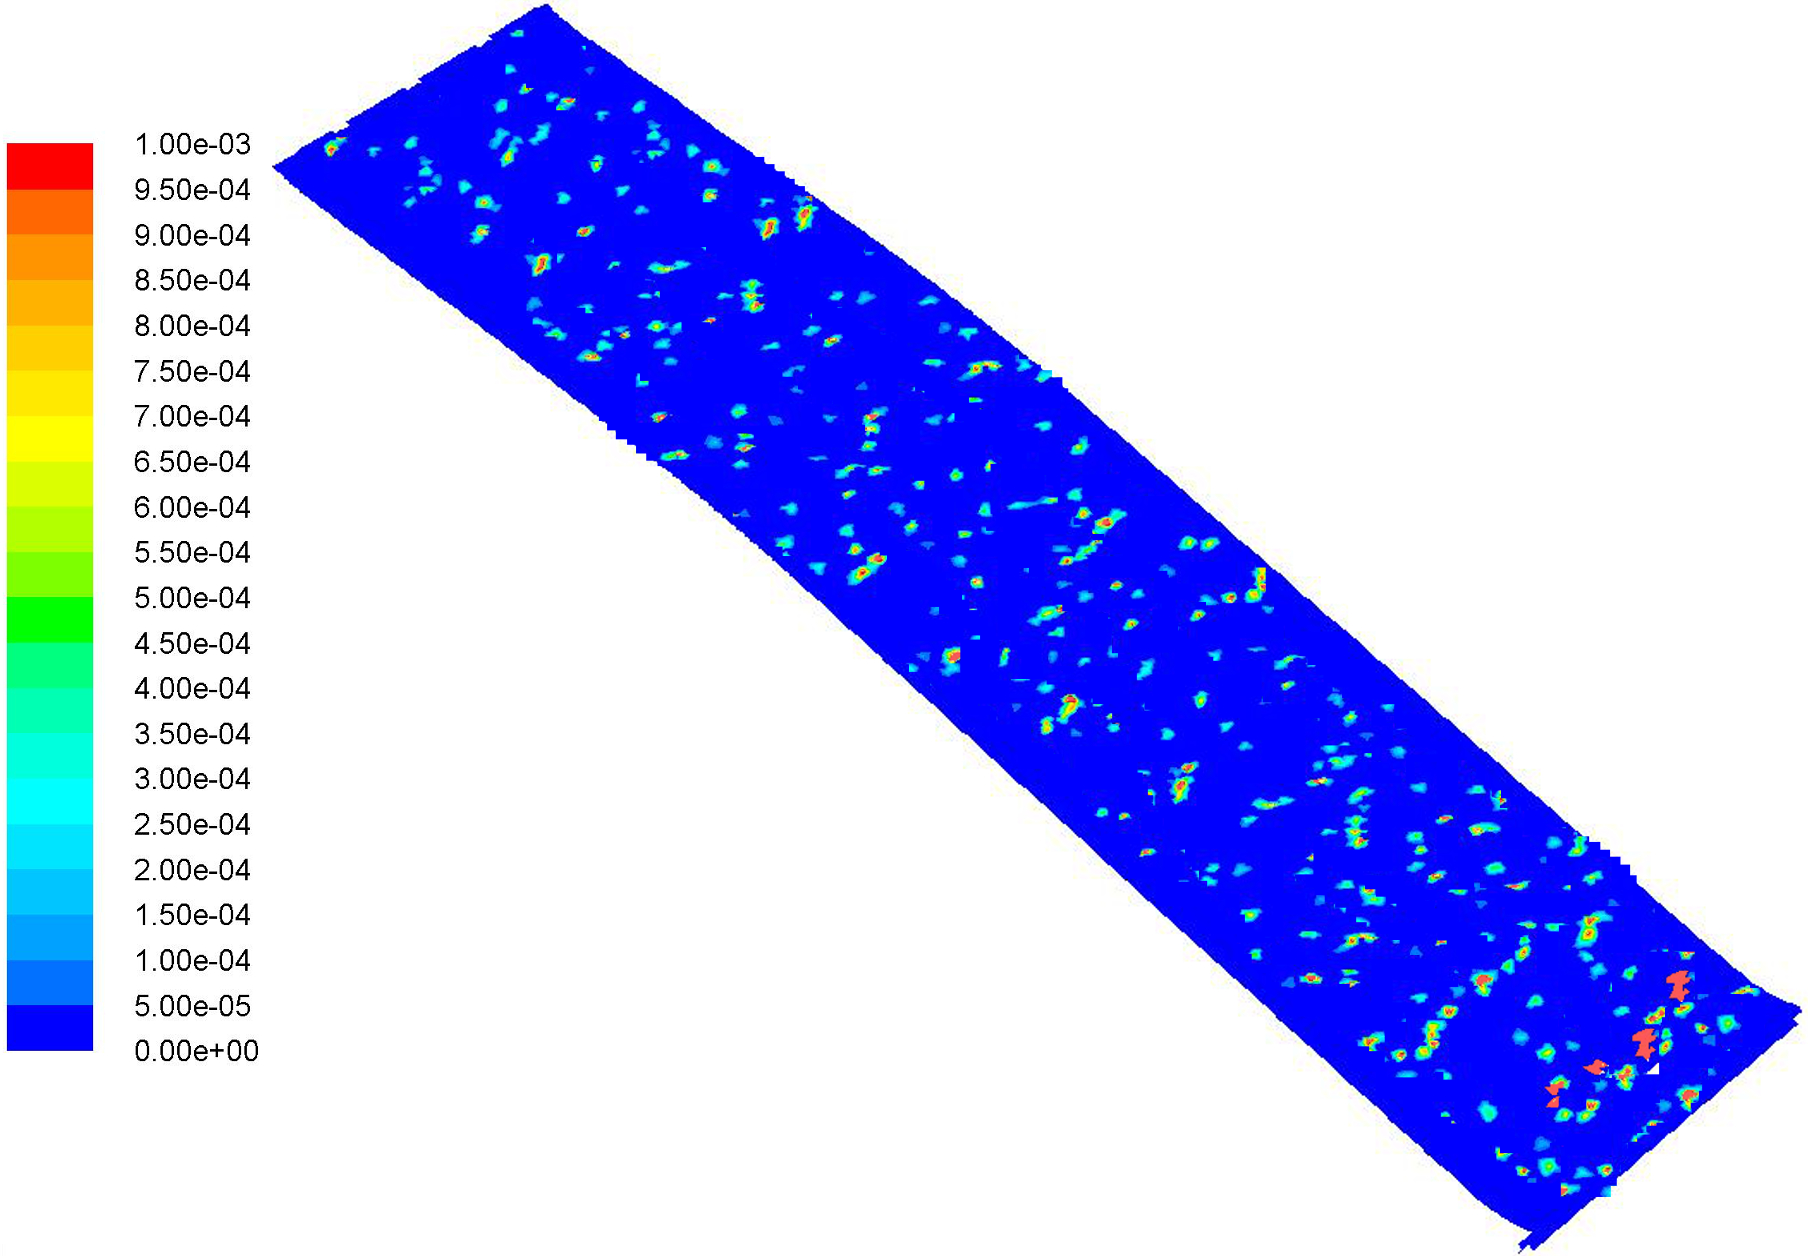
\includegraphics[width=0.44\textwidth]{figuras/erosao_dpm}} \quad
		\subfigure[Dom�nio com rugosidade num�rica.]{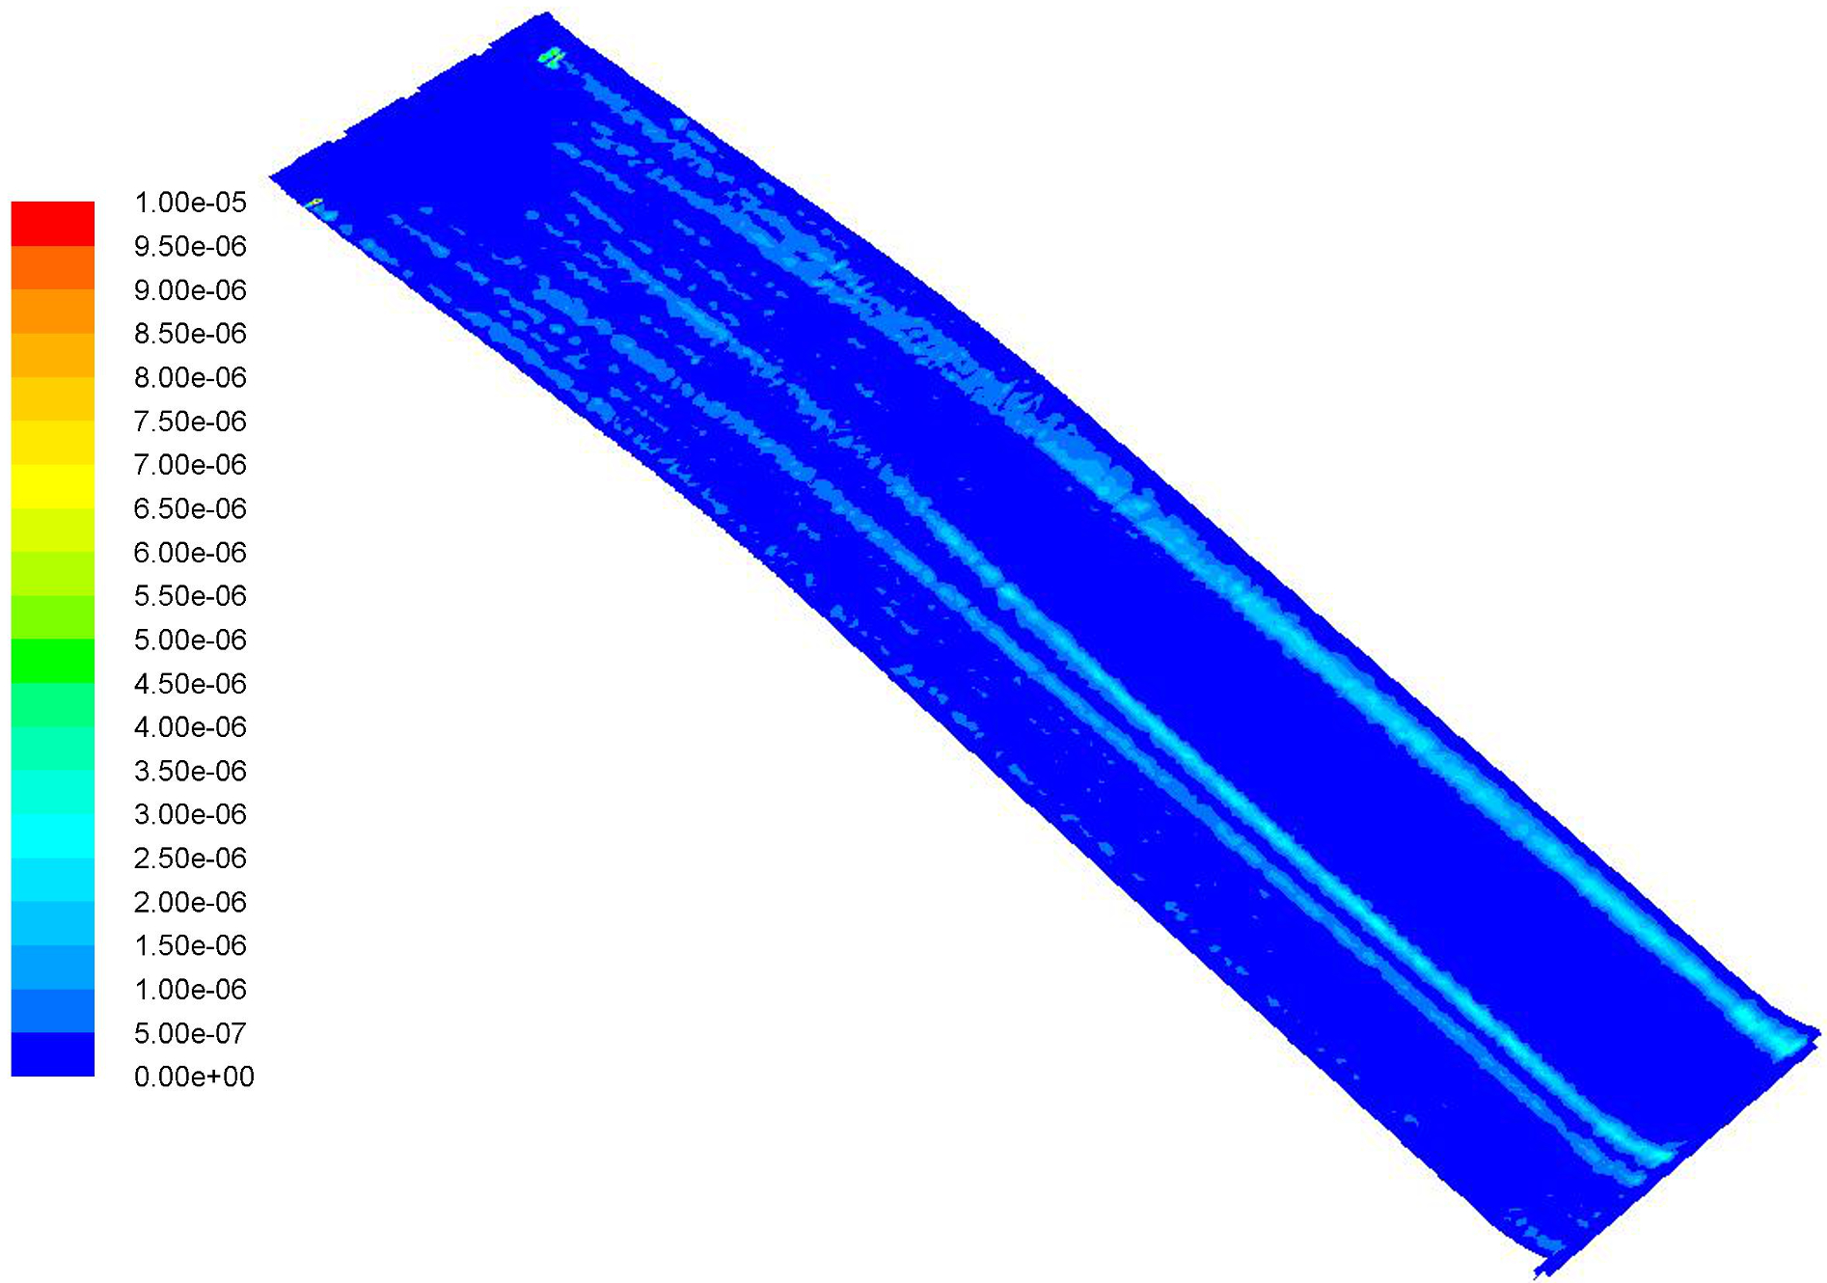
\includegraphics[width=0.44\textwidth]{figuras/erosao}} \\
  	\subfigure[Alguns pontos de desgaste georreferenciados.]{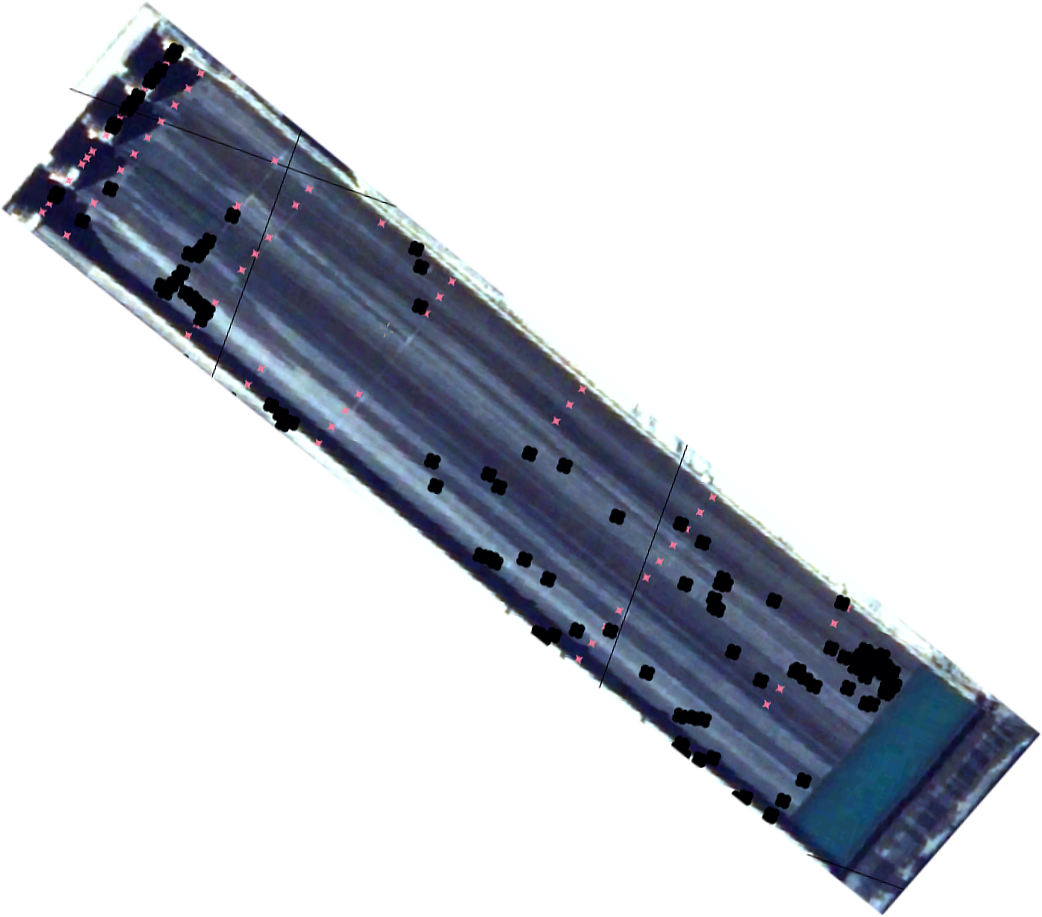
\includegraphics[width=0.4\textwidth]{figuras/pontos_erosao}}
	\caption{Resultados de simula��es e pontos amostrais de desgaste na calha direita.}
	\label{fig:compara}
\end{figure}

� relevante, pois, ao estudo da intera��o fluido-estrutura a avalia��o da influ�ncia da aplica��o de diferentes modelos de turbul�ncia no estudo de efeitos abrasivos-erosivos envolvidos no desgaste superficial de estruturas de concreto, visto a associa��o dos modelos das equa��es de momentum e de turbul�ncia no c�lculo das trajet�rias das part�culas que incidem sobre a superf�cie material, dado que esta utiliza a velocidade do fluido e a viscosidade din�mica do fluido na determina��o da velocidade da particula, que por sua vez � empregada na express�o para avaliar a taxa de abras�o-eros�o, relacionada com a avalia��o do desgaste do concreto.

Assim sendo, a proposta de trabalho aqui apresentada busca a avalia��o do emprego de diferentes modelos de turbul�ncia nos resultados de simula��es num�rico-computacionais para quantifica��o do desgaste superficial abrasivo-erosivo da calha esquerda do vertedouro. Estas atividades ser�o realizadas como parte do projeto de pesquisa de doutorado desenvolvido pelo autor, e como parte das atividades a serem desenvolvidas pelo proponente do projeto denominado ``Estudos Experimental-Num�ricos e Simula��o Computacional de Efeitos Abrasivo-Erosivos e Envelhecimento por Radia��o Ultravioleta em Reparos e Concretos Assemelhados �queles Predominantes na Calha Esquerda do Vertedouro da Barragem da Usina Hidroel�trica de Itaipu''.



%%\Huge
%
%$u_i = \bar{u}_i + u_i'$
%
%\
%
%$\phi = \bar{\phi} + \phi'$
%
%\
%
%$ SST \ \ \ k-\omega \ \ \ \ k-\epsilon \ \ \ \ LES \ \ \ \ TLES \ \ \ DNS$
%
%\
%
%$$
%\dfrac{\partial \rho}{\partial t} + \dfrac{\partial}{\partial x_i}(\rho u_i)=0
%$$
%
%\
%
%\begin{equation}
%\dfrac{1}{\rho_q}\bigg[ \dfrac{\partial}{\partial t}(\alpha_q \rho_q)+ \nabla\cdot (\alpha_q\rho_q \hat{u}_q)\ = S_{\alpha_q} \sum^n_{p=1} (\dot{m}_{pq} - \dot{m}_{qp})\bigg]
%\end{equation}
%
%$$
%\dfrac{\partial}{\partial t}(\rho \hat{u}) + \nabla \cdot (\rho \hat{u} \hat{u}) = - \nabla p + \nabla \cdot \big[\mu (\nabla \hat{u} + \nabla \hat{u}^T)\big]+ \rho g+ F
%$$

\begin{figure}
\centering
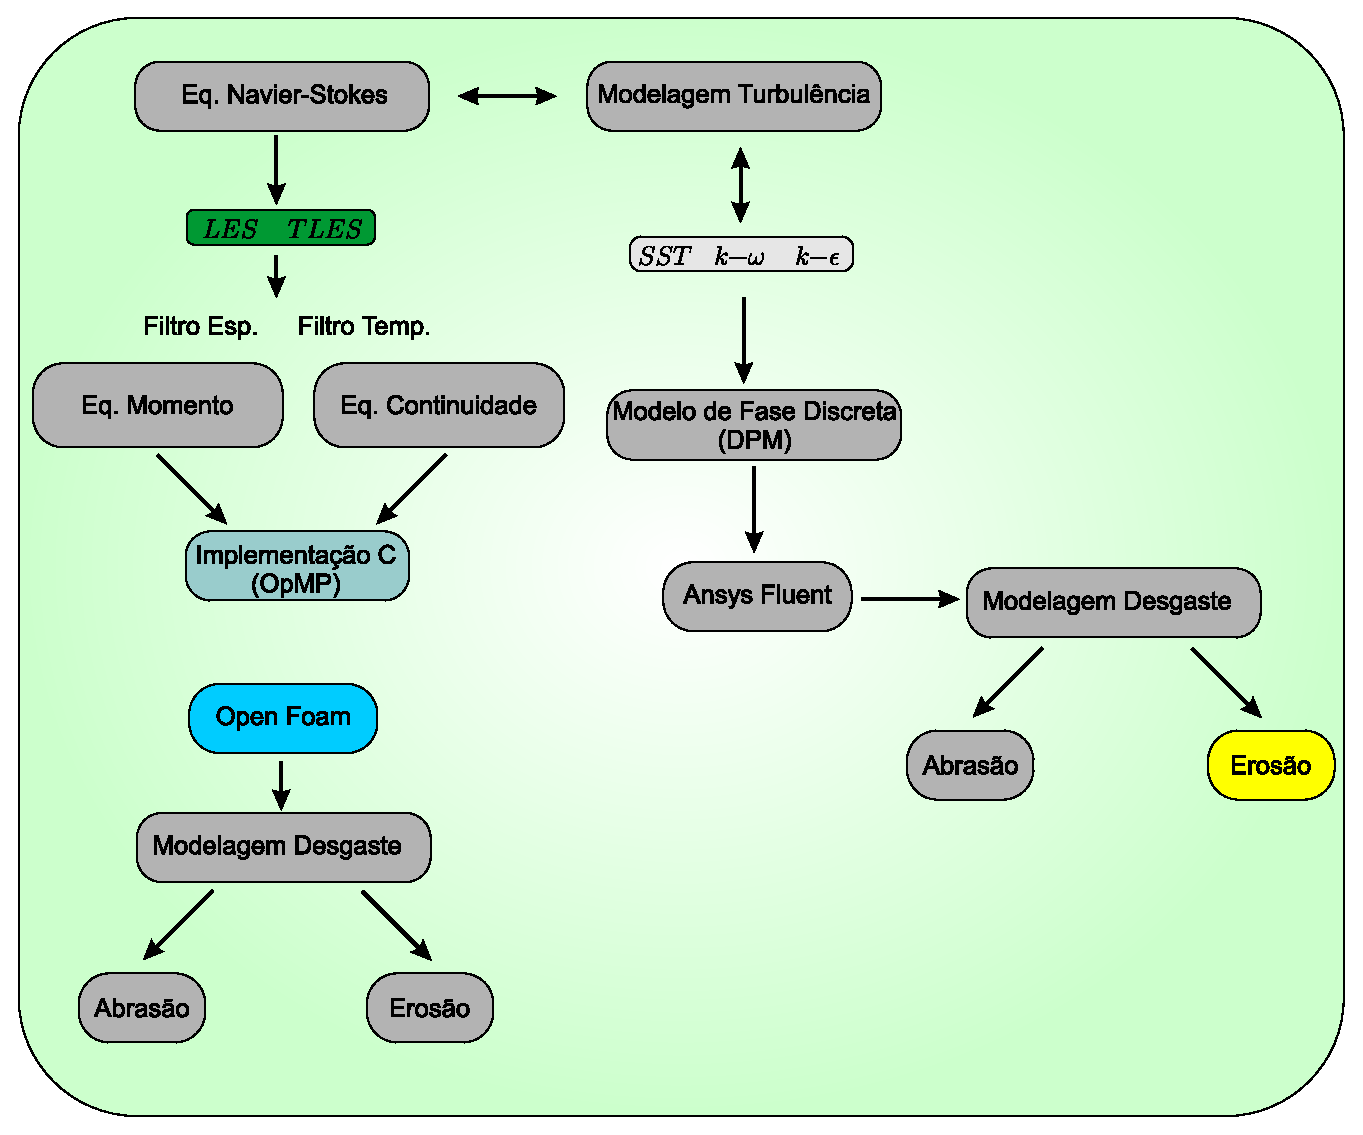
\includegraphics[width=0.8\textwidth]{figuras/fluxograma}
\end{figure}

\chapter{Turbul�ncia}
A turbul�ncia que ocorre nos fluidos est� entre os fen�menos mais complexos encontrados na natureza, sendo tridimensional e variando temporalmente. Tamb�m � caracterizado por processos n�o lineares de troca de massa, quantidade de movimento e energia, sendo essas trocas provenientes das intera��es entre estruturas de escalas variadas tanto no espa�o quanto no tempo. De forma geral, existem duas frentes de trabalho em rela��o aos estudos deste fen�meno: uma devida aos experimentalistas num�ricos e os de laborat�rio. 

Esta se��o ser� apresentada a metodologia de Simula��o de Grandes Escalas (LES) para escoamentos turbulentos, que � uma das v�rias abordagens existentes para o tratamento te�rico do tema. Tal abordagem teve in�cio em meados da d�cada de 60 com os trabalhos do meteorologista Smagorinsky, cuja motiva�� estava relacionada � simula��o das grandes escalas de escoamentos atmosf�ricos, dada a inviabilidade de simular a totalidade do espectro de escalas. Embora iniciada por Smagorinsky, foi Deardorff que ``importou`` a metodologia para problemas de engenharia \cite{Deardorff1970}. 

Deve-se ressaltar que � razo�vel o investimento em pesquisas relacionadas � compreens�o e ao controle de escoamentos turbulentos, devido � enorme quantidade de implica��es de cunho pr�tico decorrentes, que envolvem sistemas de transportes, transmiss�o e convers�o de energia, aplic��es geof�sicas, entre outras. Dentre as maiores dificuldades para o desenvolvimento da modelagem matem�tica dos escoamentos que apresentam turbu�ncia, est� a sua modelagem, o que ser� discutido nesta se��o.

A mariora dos problemas de engenharia que ocorrem na pr�tica e em grande parte dos fluxos naturais s�o turbulentos o que direciona o estudo e o desenvolvimento de t�cnicas em din�mica de fluidos computacional (CFD), a fluxos em que a turbul�ncia desempenha um papel dominante. Embora a natureza f�sica exata da turbul�ncia n�o tenha sido totalmente compreendida, ela pode ser modelada com um grau suficiente de precis�o em simula��es num�ricas \cite{Zhiyin:2015}.

Uma das principais caracter�sticas dos escoamentos turbulentos � o elevado grau de liberdade associado a este tipo de sistema din�mico. A maneira mais tradicional ou intuitiva de conduzir uma simula��o de escoamento � com aux�lio das equa��es de Navier-Stokes, e se a malha computacional for suficientemente refinada, todos os fen�menos f�sicos envolvidos ser�o resolvidos. Essa abordagem � conhecida como Simula��o Num�rica Direta (DNS), no entanto, por aspectos computacionais ela nem sempre pode ser utilizada, ficando restrita na maioria das vezes � escoamentos com baixos n�mero de Reynolds. Esse fato torna a DNS invi�vel para a maior parte dos problemas pr�ticos encontrados. Diante desta limita��o e empregando as ideias de decomposi��o das escalas de Reynolds, que Smagorinsky prop�s uma nova concep��o de modelagem, na qual � realizada uma separa��o estruturas que ocorrem em altas frequ�ncias daquelas que ocorrem em baixa frequ�ncia, ao inv�s de separar as escalas em um campo m�dio e nas suas respectivas flutua��es. Nesta metodologia, o comprimento caracter�stico do filtro (fator que determina a frequ?ncia de corte) � especificado em fun��o do tamanho da malha utilizada na discretiza��o do problema \cite{silva_freire:2002}. 

Em alguns casos, o pesquisaor pode estar interessado  no fluxo no estado estacion�rio e, portanto, n�o � necess�rio simular o fluxo instant�neo de forma detalhada, o que leva a uma grande redu��o do custo computacional. Esta � a base para a aproxima��o de Navier-Stokes baseada nas m�dias de Reynolds (RANS), onde as equa��es s�o resolvidas apenas para as quantidades m�dias, enquanto o efeito de todas as escalas de movimento turbulento instant�neo � modelado por um modelo de turbul�ncia. Esta abordagem tem sido majorit�ria nas aplica��es de industriais de CFD nas �ltimas d�cadas, devido � sua baixa exig�ncia computacional. No entanto, o conhecimento do comportamento transit�rio do fluxo � necess�rio e a abordagem RANS n�o � suficiente, e em muitos casos n�o consegue descrever o comportamento detalhado do fluxo \cite{Zhiyin:2015}.

Uma abordagem alternativa � chamada de simula��o de grandes escalas (LES), a qual foi proposta em 1963 por Smagorinsky. Esta abordagem n�o adota a abordagem convencional de RANS com tempo ou conjunto, com equa��es adicionais de transporte modeladas sendo resolvidas para obter o tensor de tens�es de Reynolds resultantes do processo de m�dia. Na LES, os movimentos em grande escala (grandes v�rtices) de fluxo turbulento s�o calculados diretamente, e apenas os movimentos de pequena escala (escala sub-malha (SGS)) s�o modelados, resultando em uma redu��o significativa no custo computacional quando comparado ao DNS. Desta forma, LES � mais precisa do que a abordagem RANS, uma vez que as grandes escalas turbulentas cont�m a maior parte da energia turbulenta e s�o respons�veis ??pela maior parte da transfer�ncia de momentum e difus�o turbulenta, e LES captura estas estruturas em detalhe completo diretamente, enquanto elas s�o modelados na abordagem RANS. Al�m disso, as pequenas escalas tendem a ser mais isotr�picas e homog�neas do que as grandes e, portanto, modelar os movimentos do SGS pode ser mais f�cil do que modelar todas as escalas dentro de um �nico modelo como na abordagem RANS \cite{Zhiyin:2015}.

A Simula��o de Grandes Escalas � considerada como uma metodologia intermedi�ria � DNS e � simula��o empregando equa��es resultantes da t�cnica de decomposi��o de Reynolds. Uma caracter�stica desta abordagem � que as estruturas turbulentas respos�veis pelo transporte de energia e quantidade de movimento s�o resolvidas diretamente por meio das equa��es filtradas, e somenteas as menores estruturas, que ocorrem com maior frequ�ncia s�o modeladas - filtro passa-baixa. Ao considerar que estruturas menores apresentem uma isotropia e homogeneidade, espera-se que os modelos sejam mais gerais e independentes dos diferentes tipos de escoamento, quando comparados � metodologia que emprega m�dias.

Ambas metodologias DNS e LES se assemelham, uma vez que ambas permitem a obten�a� de resultados tridimensionais e transientes das equa��es de Navier-Stokes. Embora seja necess�rio uma malha tamb�m refinida para LES, nesta abordagem � poss�vel resolver escoamentos com altos n�mero de Reynolds, devido ao processo de separa��o das escalas utilizado e ao processo de modelagem dos tensores -sub-malha que s�o obtidos adicionalmente.

Quando o m�todo de volumes finitos � empregado para resolver as equa��es governantes numericamente, as equa��es s�o integradas sobre volumes de controle, equivalentes a convolu��o com um filtro de chap�u alto, portanto n�o h� necessidade de aplicar explicitamente um filtro � equa��o instant�nea e isso � chamado filtragem impl�cita. No entanto, vale a pena salientar que existe potencialmente uma grande defici�ncia ou dificuldade na filtragem impl�cita, ou seja, uma verdadeira malha resultados independentes nunca podem ser alcan�ados como com o refinamento de malha, menor escala movimentos s�o resolvidos e se um continua a refinar a Malha, em seguida, eventualmente, um DNS � realizado, e n�o um LES. Em outras palavras, quando a filtragem impl�cita � empregada, � quase imposs�vel distinguir entre erros num�ricos e de modelagem e, portanto, pro�be a an�lise �til de esquemas num�ricos.


\section{M�dias e filtros}
No caso de escoamento de fluidos, a turbul�ncia origina-se da instabilidade de camadas de cisalhamento, que surge no momento em que os efeitos n�o-lineares s�o dominantes, o que � caracterizado por elevados n�meros de Reynolds. Na maioria das vezes, � de interesse avaliar as propriedades m�dias dos escoamentos turbulentos. Para isso, decomp�e-se cada grandeza f�sica $u$ na soma de um campo m�dio $\bar{u}$ e uma componente de flutua��o turbulenta $u'$, cuja m�dia � considerada nula. Assim os campos de velocidade, press�o e densidade s�o escritos como em \cite{pontes:2016}:
\begin{equation}
 \label{eq:media}
  u_i = \bar{u}_i + u_i' \qquad p = \bar{p} + p' \qquad \rho = \bar{\rho} + \rho_0'
\end{equation}
Como apresentado em \cite{pontes:2016} existem diversas formas de definir as grandezas m�dias e as flutua��es, sendo que as propriedades dessas grandezas dependem da sua defini��o. 

\subsection{M�dias de Reynolds}
As m�dias de Reynolds incluem as m�dias de conjunto, as m�dias temporais e as m�dias espaciais. Se o escoamento � quase estacion�rio, m�dias com rela��o ao tempo podem ser utilizadas. No caso da turbul�ncia homog�nea, as m�dias espaciais podem ser tomadas e para os  demais casos, pode ser necess�rio que as m�dias sejam obtidas sobre um grande n�mero de experimentos possuindo as mesmas condi��es iniciais e de contorno, o que nos remete ao \textit{valor esperado} ou \textit{esperan�a matem�tica} da vari�vel.

Ao tratar um processo estacion�rio e homog�neo, essas tr�s m�dias s�o id�nticas, o que � conhecido como hip�tese erg�tica. Simula��es que empregam as vari�veis das Equa��es de Navier-Stokes promediadas por Reynolds s�o denominadas de RANS (Reynolds-averaged Navier-Stokes). 

A m�dia temporal para uma turbul�cia estacion�ria � como:
\begin{equation}
 \label{eq:media_temporal}
  \bar{U}^t = \lim_{T \to \infty} \dfrac{1}{2T} \int^T_{-T} U(x_0,t) dt
\end{equation}

A m�dia espacial para uma turbul�cia homog�nea � expressa por:
\begin{equation}
 \label{eq:media_espacial}
  \bar{U}^s = \lim_{X \to \infty} \dfrac{1}{2X} \int^X_{-X} U(x,t_0) dx
\end{equation}

O valor esperado para uma repeti��o de N experimentos:
\begin{equation}
 \label{eq:media_espacial}
  \bar{U}^e = \lim_{N \to \infty} \dfrac{1}{N} \sum^N_1 U_n(x_0,t_0) 
\end{equation}

Obviamente os escoamentos de real interesse n�o s�o estacion�rios nem homog�neos. Al�m disso, por motivos pr�ticos n�o � poss�vel obter a m�dia para valores infinitos de $X$, $T$ e $N$. Deve-se ent�o determinar um intervalo adequado que represente o fen�meno em estudo, ao qual decorrer� a m�dia.

Como discutido em \cite{atila:2002} a t�cnica de passagem da m�dia de Reynolds consiste de duas etapas: na primeira, as vari�veis presentes nas equa��es do movimento s�o decompostas em termos m�dios e de flutua��es; na segunda, deve-se aplicar o operador m�dia temporal sobre um intervalo de tempo finito nos termos resultantes.

As grandezas que caracterizam o campo de um escoamento s�o escritas para o precesso de decomposi��o como:
\begin{equation}
 \label{eq:grandezas_decompostas}
 \begin{split}
  u_i & = \bar{u}_i + u_i'\\
  p & = \bar{p} + p'\\
  \rho & = \bar{\rho} + \tilde{\rho}  
 \end{split}
\end{equation}
em que $u_i$ representa as componentes da velocidade nas $i$ dire��es, $p$ � a press�o e $\rho$ � a massa espec�fica. Por nota��o, as flutua��es de densidade foram designadas por $\rho'$.

Como j� apresentado, a equa��o de conserva��o de massa ou equa��o da continuidade para um escoamento incompress�vel pode ser escrita como:
\begin{equation}
 \label{eq:conservacao}
 \dfrac{\partial \rho}{\partial t} + \dfrac{\partial}{\partial x_j}(\rho u_j) = 0
\end{equation}

Empregando as express�es m�dias para $u$ e $\rho$, em \eqref{eq:conservacao} tem-se:
\begin{equation}
 \label{eq:conservacao_media}
 \dfrac{\partial}{\partial t} (\bar{\rho} + \tilde{\rho})  + \dfrac{\partial}{\partial x_j}\big((\bar{\rho} + \tilde{\rho})(\bar{u}_i + u_i')\big) = 0
\end{equation}


\subsection{Separa��o de escalas}
As equa��es que governam o escoamento de fluidos incompress�veis s�o especificadas basicamente pelas equa��es de conserva��o da massa e da quantidade de movimento, expressas respectivamente, por:
\begin{equation}
 \label{eq:cons_massa_mom}
 \begin{split}
  \dfrac{\partial u_i}{\partial x_i } & = 0 \\
  \dfrac{\partial u_i}{\partial t} + \dfrac{\partial }{\partial x_j}(u_iu_j) & = -\dfrac{1}{\rho_0}\dfrac{\partial p}{\partial x_i}+ \dfrac{\partial }{\partial x_j}\left(\nu\dfrac{\partial u_i}{\partial x_j}\right)  
 \end{split}
\end{equation}
em que $i,j = 1,2,3$, $u$ � a velocidade $t$ � o tempo, $p$ � a press�o, $\rho_0$ a densidade e $\nu$ a viscosidade do fluido. Como observado, esse sistema apresenta 4 equa��es e 4 inc�gnitas, constituindo um sistema de equa��es fechado. A solu��o direta deste sistema de equa��es � poss�vel somente para baixos n�meros de Reynolds, e em escoamentos com elevados n�meros de Reynolds uma alternativa � solu��o � o processo de filtragem e de separa��o de escalas. Para isto, as vari�veis presentes nas referidas equa��es governantes devem ser separadas em uma parcela denominada de grandes escalas $\bar{f}(\vec{x},t)$ e em outra parte denominada sub-malha $f'(\vec{x},t)$, de forma que:
\begin{equation}
 \label{eq:les}
 f(\vec{x},t) = \bar{f}(\vec{x},t) + f'(\vec{x},t)
\end{equation}
em que a parte filtrada � definida como:
\begin{equation}
 \label{eq:filtro}
 \bar{f}(\vec{x},t) = \int_D f(\vec{x},t)G(\vec{x}-\vec{x}') d\vec{x}'
\end{equation}
onde $G(\vec{x})$ � a fun��o filtro e pode ser definida de diversas formas. Uma das mais frequentes fun��es filtro encontradas na literatura � expressa por:
\begin{equation} 
 \label{eq:funcao_filtro}
 G(\vec{x}) = \left\{
 \begin{array}{cc}
  1/\Delta^3 	& \text{ se } |\vec{x}| \leq \Delta/2\\
  0		& \text{ se } |\vec{x}| > \Delta/2\\
 \end{array}
 \right.
\end{equation}
em que $\Delta$ � o tamanho caracter�stico do filtro, e caracteriza a frequ�ncia de corte da filtragem. 



\section{Simula��o de grandes escalas - LES}
A simula��o de grandes escalas (LES) foi originalmente proposta para simular fluxos atmosf�ricos na d�cada de 1960 e partir de ent�o, tornou-se uma das metodologias mais promissoras e bem-sucedidas para a simula��o de escoamentos ou fluxos turbulentos. Atualmente � poss�vel simular fluxos complexos e de real interesse em engenharia empregando a t�cninca LES. No entanto, ainda existem desafios significativos para que esta abordagem atinja um n�vel de maturidade para sua ampla dissemina��o em aplica��es de engenharia e de ind�stria \cite{Zhiyin:2015}



\chapter{Instala��o e Configura��o do PETSC}
Esta se��o � breve e tem como objetivo auxiliar na instala��o e configura��o do pacote de ferramentas PETSC, seguindo o manual do software. Informa��es adicionais podem ser obtidas diretamente no site do desenvolvedor da ferramenta: \url{https://www.mcs.anl.gov/petsc/}. 

Nesta se��o ser�o apresentados tamb�m alguns requisitos computacionais necess�rios � implementa��o dos m�todos num�ricos e resolu��o das equa��es discretizadas. Tamb�m ser� exibido uma introdu��o, instala��o e configura��o da biblioteca PETSC para o sistema Linux Ubuntu 16.04. PETSc (Portable, Extensible Toolkit for Scientific Computation), � um conjunto de estruturas de dados e rotinas para solu��o paralela de aplica��es cient�ficas modeladas por meio de equa��es diferenciais parciais. 

Para instala��o do PETSc � necess�rio a realiza��o do download da distribui��o mais atual do pacote, o que pode ser obtido no link \url{https://www.mcs.anl.gov/petsc/download/index.html}. Ap�s a obten��o do arquivo \texttt{.tar.gz} � necess�rio extra�-lo em alguma pasta do computador local. Isto pode ser feito por meio do terminal e empregando o comando \texttt{tar -xf petsc-3.7.5.tar.gz}. Ap�s a extra��o, deve-se acessar a pasta que foi criada e que neste tutorial chama-se \texttt{/petsc-3.7.5.tar.gz} e executar o comando para configura��o do PETSC: 
\begin{flushleft}
 \texttt{./configure --with-cc=gcc --with-cxx=g++ --with-X=1 --with-fc=gfortran --download-mpich --download-fblaslapack}
\end{flushleft}
Esse comando, al�m de configurar o PETSC, tamb�m instala algumas ferramentas como compiladores e bibliotecas. Caso a configura��o ocorra corretamente uma mensagem semelhante � da Figura \ref{fig:install_01} deve ser exibida no terminal.
\begin{figure}[H]
 \centering
 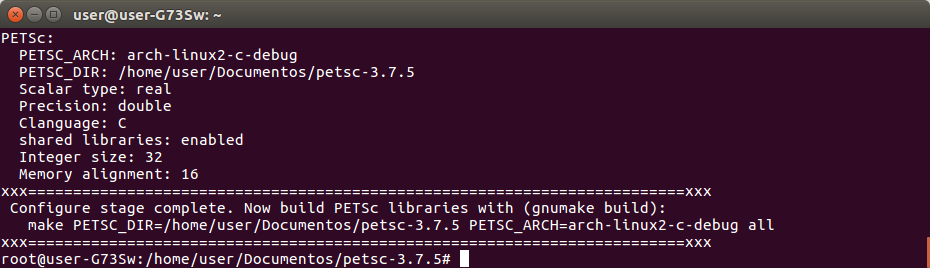
\includegraphics[width=0.7\textwidth]{figuras/install_01.png}
 \caption{Terminal configura��o PETSC.}
 \label{fig:install_01}
\end{figure}
Como indicado, o usu�rio deve em seguida executar o seguinte comando:
\begin{flushleft}
 \verb|make PETSC_DIR=/home/user/Documentos/petsc-3.7.5 PETSC_ARCH=arch-linux2-c-debug all|
\end{flushleft}
o que resultar� na seguinte Figura \ref{fig:install_02}.
\begin{figure}[H]
 \centering
 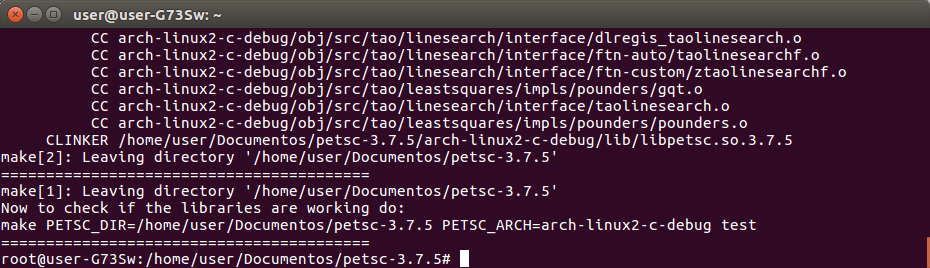
\includegraphics[width=0.7\textwidth]{figuras/install_02.png}
 \caption{Terminal configura��o PETSC.}
 \label{fig:install_02}
\end{figure}
Como indicado, o usu�rio deve verificar se as bibliotecas est�o trabalhando corretamente, por meio do comando:
\begin{flushleft}
 \verb|make PETSC_DIR=/home/user/Documentos/petsc-3.7.5 PETSC_ARCH=arch-linux2-c-debug test|
\end{flushleft}
o que resultar� na seguinte Figura \ref{fig:install_03}.
\begin{figure}[H]
 \centering
 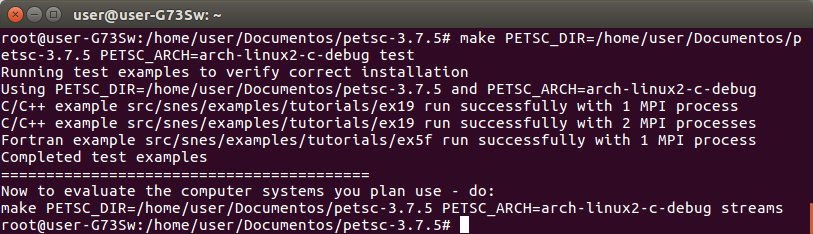
\includegraphics[width=0.7\textwidth]{figuras/install_03.png}
 \caption{Terminal configura��o PETSC.}
 \label{fig:install_03}
\end{figure}
Para finalizar a configura��o, o usu�rio deve o sistema, por meio do comando:
\begin{flushleft}
 \verb|make PETSC_DIR=/home/user/Documentos/petsc-3.7.5 PETSC_ARCH=arch-linux2-c-debug streams|
\end{flushleft}
o que resultar� na seguinte Figura \ref{fig:install_04}.
\begin{figure}[H]
 \centering
 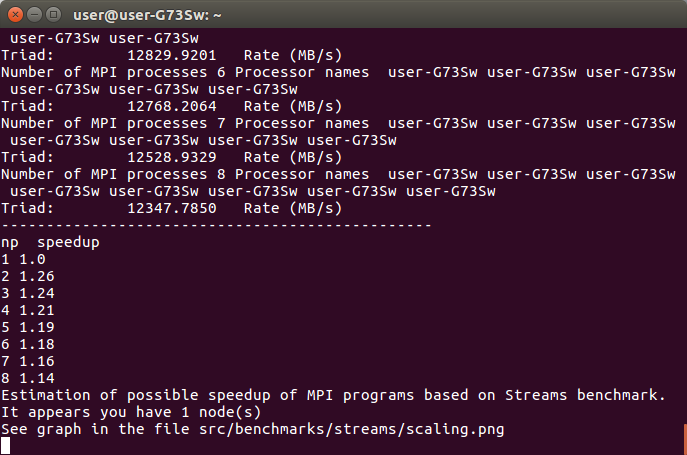
\includegraphics[width=0.6\textwidth]{figuras/install_04.png}
 \caption{Terminal configura��o PETSC.}
 \label{fig:install_04}
\end{figure}
Se a instala��o foi realizada com �xito uma janela com o speedup em fun��o do n�mero de processadores ser� exibida.
\begin{figure}[H]
 \centering
 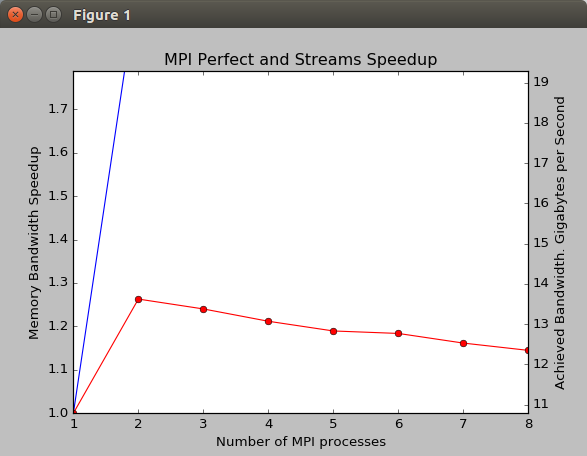
\includegraphics[width=0.6\textwidth]{figuras/install_speedup.png}
 \caption{Terminal configura��o PETSC.}
 \label{fig:install_speedup}
\end{figure}

Ao t�rmino da instala��o deve-se tamb�m configurar, via terminal, as vari�veis de ambiente \verb|PETSC_DIR=/home/user/Documentos/petsc-3.7.5| e \verb|PETSC_ARCH=arch-linux2-c-debug| com aux�lio do comando \texttt{export}. Ver Figura \ref{fig:install_environment}.
\begin{figure}[H]
 \centering
 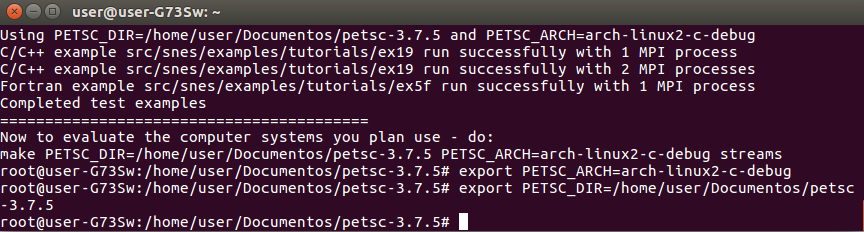
\includegraphics[width=0.7\textwidth]{figuras/install_environment.png}
 \caption{Terminal configura��o PETSC.}
 \label{fig:install_environment}
\end{figure}

Para verificar se a instala��o e configura��o foram realizadas com �xito, � poss�vel navegar at� a o diret�rio: \verb|cd /home/user/Documentos/petsc-3.7.5/src/ksp/ksp/examples/tutorials/| e executar os comandos:
\begin{flushleft}
 \verb|make ex1|
\end{flushleft}
o que resultar� na Figura \ref{fig:make_ex1}.
\begin{figure}[H]
 \centering
 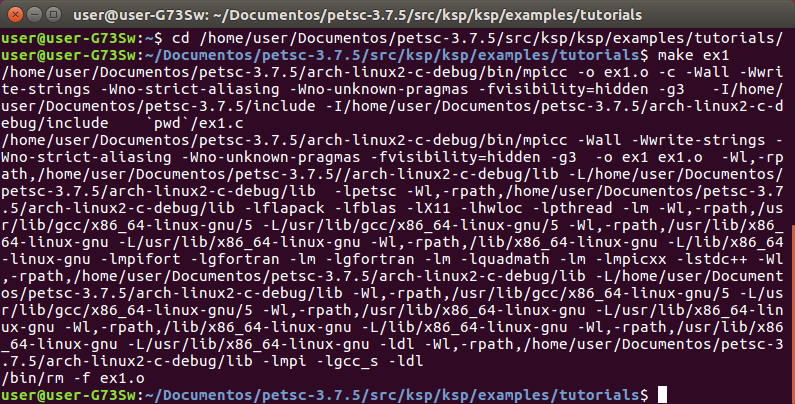
\includegraphics[width=0.7\textwidth]{figuras/make_ex1.png}
 \caption{Terminal exemplo ex1.c.}
 \label{fig:make_ex1}
\end{figure}
Para executar o c�digo acima compilado, digita-se \verb|./ex1|, o que deve resultar em algo semelhante � Figura \ref{fig:exec_ex1}.
\begin{figure}[H]
 \centering
 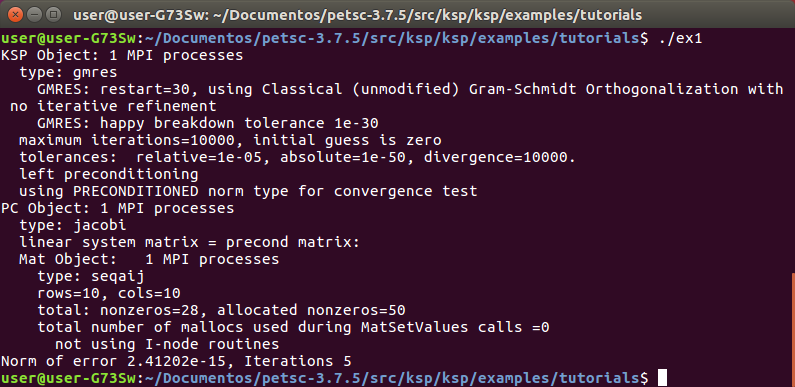
\includegraphics[width=0.7\textwidth]{figuras/exec_ex1.png}
 \caption{Execu��o do exemplo ./ex1}
 \label{fig:exec_ex1}
\end{figure}

Para uma configura�� completa do PETSC, talvez seja necess�ria a instala��o de alguns pacotes adicionais como � o caso do X11 para cria��o de janelas gr�ficas. Sua instala��o pode ser realizada via terminal com o comando: \verb|apt install libxt-dev|.

\section{Primeiros exemplos com PETSC}
Como j� mencionado o PETSC � uma suite de ferramentas que permite a solu��o de sistemas de equa��es em paralelo. Essa suite foi desenvolvida para resolu��o de Equa��es Diferenciais Parciais, em que sua resolu��o conduz � resolu��o de sistemas de equa��es de grandes dimens�es, o que demanda algoritmos eficientes e programa��o paralela. Desta forma o prop�stico da biblioteca PETSC � auxiliar na solu��o de problemas cient�ficos e de engenharia em computadores multiprocessados. O primeiro exemplo aqui ilustrado � apresentado em \cite{bueler:2017} e aproxima a constante de Euler por meio da s�rie de Maclaurin:
\begin{equation}
  \label{eq:ex_01}	
  e = \sum_{n=0}^\infty \dfrac{1}{n!} \approx 2.718281828
\end{equation}
O programa \verb|code_euler.c| , ilustrado no c�digo \ref{code:code_euler}, realiza a computa��o de cada termo da s�rie infinita em cada processo, resultando numa melhor estimativa de $e$ quando executado em v�rios processos MPI. Embora seja um exemplo ing�nuo do emprego da biblioteca PETSC, ele auxilia na compreens�o de algumas ideias envolvidas em computa��o paralela.

\lstinputlisting[language=C,caption=C�digo constante de Euler.,label=code:code_euler]{codigo/code_euler.c}

Como qualquer programa escrito em linguagem C, o c�digo � iniciado com uma fun��o chamada \texttt{main()} a qual tem os argumentos \texttt{argc} e \texttt{argv} passados via linha de comando. No exemplo ilustrado esses argumentos ser�o passados � biblioteca atrav�s da fun��o \texttt{PetscInitialize()}, e a biblioteca obt�m as informa��es passadas em linha de comando. A fun��o \texttt{main()} tamb�m tem como retorno um valor inteiro, que � igual a 0 se o programa foi executado corretamente. Al�m disso, � importante utilizar a fun��o PETSC para verica��o de erros associados � sua utiliza��o, \texttt{CHKERRQ(ierr)}, a qual retorna um valor inteiro diferente de 0 caso alguma anomalia ocorra na execu��o de alguma fun��o pertencente � biblioteca.

Como indicado no manual \cite{petsc} para compilar um arquivo que utiliza PETSC, deve-se ter no mesmo diret�rio do arquivo fonte, um arquivo \texttt{makefile}, cujo conte�do � exibido no c�digo \ref{code:make}.

\lstinputlisting[language=C]{codigo/makefile}

Ap�s ter criado o arquivo \texttt{makefile} � poss�vel compilar o c�digo programa \verb|code_euler.c| com o seguinte comando:
\begin{flushleft}
\verb|user@user-G73Sw:~$ make code_euler|
\end{flushleft}
Para executar o c�digo compilado basta digitar
\begin{flushleft}
\verb|user@user-G73Sw:~$ ./code_euler|\\
\verb|O valor da constante 'e' � aproximadamente: 1.000000000000000|\\
\verb|rank 0 did 0 flops|
\end{flushleft}
O valor obtido para $e=1.0$ � uma estimativa muito ruim, e isso pode ser melhorado com a execu��o de mais processos MPI, da seguinte forma:
\begin{flushleft}
\verb|user@user-G73Sw:~$ mpiexec -n 5 ./code_euler|\\
\verb|O valor da constante 'e' � aproximadamente: 2.708333333333333|\\
\verb|rank 0 did 0 flops|\\
\verb|rank 1 did 0 flops|\\
\verb|rank 2 did 1 flops|\\
\verb|rank 3 did 2 flops|\\
\verb|rank 4 did 3 flops|\\
\end{flushleft}
Executando o mesmo programa em 10 processos, obtemos uma boa aproxima��o constante
\begin{flushleft}
\verb|user@user-G73Sw:~$ mpiexec -n 10 ./code_euler|\\
\verb|O valor da constante 'e' � aproximadamente: 2.718281525573192|\\
\verb|rank 0 did 0 flops|\\
\verb|.....|\\
\end{flushleft}
Com base na execu��o dos 10 processos acima, pode-se imaginar que o c�digo tenha sido escrito usando um cluster com no m�nimo 10 processadores f�sicos. Na verdade, esses 5 e 10 processos funcionam muito bem em um computador pessoal com 2 n�cleos (processodor i3 2120). Os processos MPI s�o criados conforme necess�rio, usando um recurso antigo de sistemas operacionais: multitarefa. Obviamente a acelera��o real do paralelismo (speedup) � outra quest�o.

No exemplo do programa \verb|code_euler.c|, cada processo MPI calcula o termo $1/n!$, onde $n$ � o retorno de \verb|MPI_Comm_rank()|. � importante notar que \verb|PETSC_COMM_WORLD| � um comunicador MPI contendo todos os processos gerados usando \verb|mpiexec -n N| na linha de comando. Uma chamada para \verb|MPI_Allreduce()| calcula a soma parcial de express�o \eqref{eq:ex_01} e envia o resultado de volta para cada processo. Esses usos diretos da API MPI s�o uma parte (relativamente pequena) do uso do PETSc, mas ocorrem porque o PETSc geralmente evita a duplica��o da funcionalidade MPI.

A estimativa calculada de $e$ � impressa de uma s� vez. Al�m disso, cada processo tamb�m imprime seu \verb|rank| e o trabalho que ele fez. O comando de impress�o formatado \verb|PetscPrintf()|, semelhante ao \verb|fprintf()| da biblioteca padr�o C, � chamado duas vezes no c�digo. Na primeira vez MPI usa o comunicador \verb|PETSC_COMM_WORLD| e a segunda vez \verb|PETSC_COMM_SELF|. O primeiro desses trabalhos de impress�o �, portanto, coletivo em todos os processos, e apenas uma linha de sa�da � produzida, enquanto a segunda � individual para cada processo e obtemos $n$ linhas impressas. As linhas de sa�da \verb|PETSC_COMM_SELF| podem aparecer em ordem aparentemente aleat�ria uma vez que a impress�o ocorre na ordem que essa classifica��o encontra o comando \verb|PetscPrintf()| no c�digo.

Todo programa ou parte de comando que utiliza a biblioteca PETSC, deve iniciar e terminar com as fun��es \verb|PetscInitialize()| e \verb|PetscFinalize()|, respectivamente. Observa-se que o �ltimo argumento da fun��o \verb|PetscInitialize(&argc, &argv, NULL, help)| fornece uma string que informa ao usu�rio uma breve descri��o do programa, e pode ser visualizada atrav�s do comando:
\begin{flushleft}
\verb|user@user-G73Sw:~$ ./code_euler --help|\\
\verb|O valor da constante 'e' � aproximadamente: 2.718281525573192|\\
\verb|rank 0 did 0 flops|\\
\verb|.....|\\
\end{flushleft}

\subsection{Objetos do tipo vetores e matrizes em PETSC}
A maioria dos m�todos de resolu��o num�rica de equa��es diferenciais cumlmina na solu��o de sistemas lineares de dimens�o finita. Como esses sistemas lineares se tornam representa��es mais precisas do PDE � medida que seu tamanho vai para o infinito, busca-se resolver os maiores sistemas lineares que a tecnologia de computa��o dispon�vel possa ser capaz de suportar. Resolver tais sistemas lineares, usando algoritmos que t�m o potencial de escalar para tamanhos muito grandes - t�o grandes, por exemplo, que a solu��o vetorial do sistema deve ser distribu�da atrav�s de muitos processadores at� mesmo se encaixar na mem�ria - representa a tecnologia de n�cleo em PETSc.

Uma observa��o a ser feita, � que muitas das PDEs discretizadas geram sistemas lineares com estrutura explor�vel, especialmente a esparcidade, o que significa que h� poucas entradas diferentes de zero por linha na matriz. Para que os m�todos convirjam, tamb�m precisa haver outra estrutura no sistema linear, tal como a regularidade das entradas de matrizes que surgem da suavidade dos coeficientes na PDE. A aplica��o ing�nua de m�todos diretos � na maioria das vezes, muito lenta.

O c�digo exibido a seguir ilustra um exemplo da cria��o de um vetor $10\times1$ em PETSc. 

\lstinputlisting[language=C]{codigo/build_vector.c}

Para compilar o c�digo acima, deve-se alterar o arquivo \verb|makefile| para deix�-lo semelhante ao apresentado abaixo:

\lstinputlisting[language=C]{codigo/makefile}

Em seguida o c�digo � compilado e executado atrav�s dos comandos:
\begin{flushleft}
\verb|user@user-G73Sw:~$ make build_vector|\\
\verb|user@user-G73Sw:~$ ./build_vector -vec_view|\\
\verb|Mat Object: 1 MPI processes|\\
\verb|type: seqaij|\\
\verb|11.|\\
\verb|7.|\\
\verb|5.|\\
\verb|3.|\\
\verb|6.|\\
\verb|11.|\\
\verb|7.|\\
\verb|5.|\\
\verb|3.|\\
\verb|6.|
\end{flushleft}

A seguir � apresentado um exemplo simples de como preencher uma matriz $4 \times 4$, usando um loop 'for' sobre o �ndice de linha $i$. O programa � denominado de \verb|build_matrix.c|:

\lstinputlisting[language=C]{codigo/build_matrix.c}

O resultado ou a matriz criada pode ser visualizada de v�rias formas, e aqui faremos duas visualiza��es uma no formato esparso e outra mostrando todos os seus elementos.
\begin{flushleft}
\verb|user@user-G73Sw:~$ ./build_matrix -mat_view|\\
\verb|Mat Object: 1 MPI processes|\\
\verb|type: seqaij|\\
\verb|row 0: (0, 1.)  (1, 2.)  (2, 3.)  (3, 0.) |\\
\verb|row 1: (0, 2.)  (1, 1.)  (2, -2.)  (3, -3.) |\\
\verb|row 2: (0, -1.)  (1, 1.)  (2, 1.)  (3, 0.) |\\
\verb|row 3: (0, 0.)  (1, 1.)  (2, 1.)  (3, -1.) |

\verb|user@user-G73Sw:~$ ./build_matrix -mat_view ::ascii_dense|\\
\verb|Mat Object: 1 MPI processes|\\
\verb|type: seqaij|\\
\verb| 1.00000e+00  2.00000e+00  3.00000e+00  0.00000e+00 |\\
\verb| 2.00000e+00  1.00000e+00 -2.00000e+00 -3.00000e+00 |\\
\verb|-1.00000e+00  1.00000e+00  1.00000e+00  0.00000e+00 |\\
\verb| 0.00000e+00  1.00000e+00  1.00000e+00 -1.00000e+00 |
\end{flushleft}

� poss�vel tamb�m salvar a matriz impressa no terminal atrav�s do comando:
\begin{flushleft}
\verb|./build_matrix -mat_view ascii:build_matrix.txt:ascii_dense|.
\end{flushleft}

Como descrito em \cite{bueler}, embora PETSC seja escrito em C, e n�o em C ++, ela � uma biblioteca orientada a objetos. Para construir o nosso primeiro c�digo PETSc para resolver um sistema linear, vamos usar os tipos de dados \verb|Vec| e \verb|Mat|, que s�o essencialmente objetos, que possuem vetores e matrizes. O exemplo a seguir descreve a solu��o do sistema linear:
\begin{equation}
  \label{eq:sistema_01}
    \left[
    \begin{array}{cccc}
     1 & 2 & 3 & 0 \\
     2 & 1 & -2 & -3 \\
     -1 & 1 & 1 & 0\\
     0 & 1 & 1 & -1 
     \end{array} 
     \right]
     \left[
     \begin{array}{l}
      x_0\\
      x_1\\
      x_2\\
      x_3
     \end{array}
     \right] = \left[
     \begin{array}{l}
      7\\
      1\\
      1\\
      3
     \end{array}
     \right] 
\end{equation}

Um objeto KSP resolve o sistema linear, com o algoritmo de solu��o espec�fico escolhido apenas em tempo de execu��o. O c�digo fonte que cont�m o programa para resolver o sistema \eqref{eq:sistema_01} � apresentado a seguir:

\lstinputlisting[language=C]{codigo/solve_linear_ksp.c}

O resulta final da execu��o do programa \verb|solve_linear_ksp.c| �:
\begin{flushleft}
\verb|user@user-G73Sw:~$ ./solve_linear_ksp|\\
\verb|Vec Object: 1 MPI processes|\\
\verb|type: seq|\\
\verb|1.|\\
\verb|0.|\\
\verb|2.|\\
\verb|-1.|
\end{flushleft}

O c�digo \verb|solve_linear_ksp.c| apresentou a solu��o de um sistema com dimens�o fixa, no entanto pode ser necess�rio, alterar essa dimens�o em tempo de execu��o, como � o caso do pr�ximo exemplo. Ele resovle um sistema de equa��o com tamanho arbitr�rio e definido no momento da execu��o, atrav�s de um valor inteiro passado na fun��o \verb|PetscOptionsXXX()|. Al�m disso, nesse exemplo ser�o vistos algumas formas de manipula��o de vetores como soma e determina��o da sua norma euclidiana, utilizando \verb|VecAXPY| e \verb|VecNorm|, respectivamente. O programa � ilustrado no c�digo..................

\lstinputlisting[language=C]{codigo/solve_linear_arbitrary.c}

� importante destacar que embora o tamanho do sistem seja arbitr�rio, ele sempre ter� a forma tridiagonal, com valores 3 na diagonal principal e valor -1 na diagonal superior e inferior. 

O primeiro novo recurso usado neste c�digo � \verb|PetscOptionsBegin()| e \verb|PetscOptionsEnd()|, ou seja, a chamada para \verb|PetscOptionsInt()|. O in�cio do m�todo define um prefixo \verb|-tri_| para que a nova op��o criada seja distinguida das muitas op��es integradas do PETSc que come�am por exemplo com \verb|-ksp_| ou \verb|-vec_| ou algo do tipo. Aqui \verb|PetscOptionsInt()| cria a op��o \verb|-tri_m| para que o usu�rio possa definir a vari�vel $m$ e deixa como padr�o $m = 4$ inalterado se a op��o n�o for definida na execu��o. 

Ap�s configurar a nova op��o em \verb|solve_linear_arbitrary.c| a solu��o num�rica \verb|Vec x| � criada exatamente como fizemos no �ltimo exemplo. Mas agora tamb�m � necess�rio criar \verb|Vec s|,  \verb|Vec b| e \verb|Vec xexact|. O primeiro vetor � o lado direito do sistema linear e este �ltimo mant�m a solu��o exata para o sistema linear para que seja poss�vel avaliar o erro associado � solu��o num�rica.

Em seguida, deve-se montar a matriz A, que como mencionado � uma matriz tridiagonal. � importante mont�-la de forma eficiente em paralelo, algo que ser� relevante na resolu��o de equa��es diferenciais 2D e 3D posteriormente. No entanto, somente quando o \verb|solve_linear_arbitrary.c| � executado, sabemos quantos processos est�o em uso. O m�todo \verb|MatGetOwnershipRange()| informa o programa, executando em um determinado processo (rank), quais linhas ele possui localmente. %No caso de muitas matrizes estruturadas como esta, pode-se evitar toda comunica��o entre processos, reunindo exatamente as linhas que possu�mos.

Como observado no in�cio do c�digo \verb|solve_linear_arbitrary.c|, chamamos \ fun��o \verb|MatGetOwnershipRange(A, &Istart, &Iend)| para obter os �ndices de linha inicial e final para o processo local. Estes �ndices s�o usados como limites no loop 'for' que preenche as linhas da matriz localmente. utiliza-se  \verb|MatSetValues()| para realmente definir as entradas da matriz  A e \verb|MatAssemblyBegin/End()| para completar a montagem de A. 

Adicionalmente, � necess�rio montar o lado direito do sistema linear e tamb�m a solu��o exacta para o sistema linear $(A \,xexato = b)$. A maneira mais simples de fazer isso, � escolher uma solu��o exata, e em seguida, calcular $b$, multiplicando A pela solu��o exata. Assim, definimos valores para \verb|xexact|. Em seguida calculamos $b$ com aux�lio da fun��o \verb|MatMult(A, xexact, b)|. 

Como em vecmatksp.c criamos o objeto KSP e ent�o chamamos o solver \verb|KSPSolve()| para resolver aproximadamente $A x = b$. A op��o \verb|-ksp_monitor| imprime a norma residual $||b - Ax||_2$ em tempo de execu��o. Neste caso, tamb�m queremos ver que o erro real $||x - x_{ex}||_2$ � pequeno quando o solver KSP � concluido. Assim, depois de obter x do KSPSolve (), calculamos o erro com os c�digos:
\begin{flushleft}
\verb|VecAXPY(x,-1.0,xexact)| : $x \leftarrow -1.0 x_{ex}+x$\\
\verb|Vecnorm(x,NORM_2,&errnorm)| : \verb|errnorm|  $\leftarrow  ||x||_2$\\
\end{flushleft}
Obviamente o sistema linear resolvido neste exemplo � f�cil de resolver por ser tridiagonal, sim�trico, diagonal-dominante e positivo definido. 
Pode-se verificar o tempo necess�rio para resolu��o do sistema com aux�lio do comando \verb|time|, como segue:
\begin{flushleft}
\verb|user@user-G73Sw:~$ time ./solve_linear_arbitrary -tri_m 1000000|\\
\verb|error for m = 1000000 system is (x-xexact)_2 = 4.8e-11|\\
\verb|real	0m1.814s|\\
\verb|user	0m1.772s|\\
\verb|sys	0m0.040s|
\end{flushleft}
Somente o tempo 'real' deve ser considerado. Note a diferen�a ao executar o mesmo c�digo com $m=10000000$.
\begin{flushleft}
\verb|user@user-G73Sw:~$ time ./solve_linear_arbitrary -tri_m 10000000|\\
\verb|error for m = 10000000 system is (x-xexact)_2 = 3.5e-10|\\
\verb|real	0m17.154s|\\
\verb|user	0m17.971s|\\
\verb|sys	0m0.140s|
\end{flushleft}
A princ�pio um sistema de equa��es contendo $10^7$ vari�veis parece ser grande. Mas pensando numa simula��o tridimensional da equa��o de Navier-Stokes em um dom�nio c�bico de 1 metro de lado e com espa�amento de malha igual a 0.01 m (1cm), isso geraria um sistema de equa��es dessa ordem de grandeza. Agora, o programa ser� executado empregando 8 processos.
\begin{flushleft}
\verb|user@user-G73Sw:~$ time mpiexec -n 8./solve_linear_arbitrary -tri_m 10000000|\\
\verb|error for m = 10000000 system is (x-xexact)_2 = 9.9e-11|\\
\verb|real	0m5.484s|\\
\verb|user	0m38.976s|\\
\verb|sys	0m2.260s|
\end{flushleft}
Como esperado, o tempo de execu��o caiu de 17 para 5 segundos, indicando um speedup de:
\begin{equation}
  546546
\end{equation}

\section{A equa��o de Poisson em uma malha estruturada}
Esta se��o � dedicada a resolu��o num�rica do problema de Poisson em um quadrado. Este � um problema que permite compreender partes essenciais  da implementa��o de c�digos empregando a biblioteca PETSc. A discretiza��o da EDP gera um sistema linear que � mais interessante do que o sistema tridiagonal que foi resolvido anteriormente. Ser� construi�da uma malha estruturada usando um objeto \verb|DMDA|, que ser� introduzido nesta  se��o, e depois ser� montada uma matriz em paralelo com base nessa malha. Por �ltimo o sistema linear resultante ser� resovido em paralelo usando um objeto \verb|KSP| \cite{petsc-user-ref}.

Neste exemplo a equa��o de Poisson ser� resolvida numa regi�o quadrada aberta, $S, (0,1)\times(0,1)$ cujo contorno � representado por $\partial S$. O problema � ilustrado na Figura \ref{fig:poisson} e formulado em \eqref{eq:poisson}.
\begin{equation}
 \label{eq:poisson}
 \begin{split}
  -\nabla^2u & = f \quad \text{em } S\\
  u & = 0 \quad \text{em } \partial S
  \end{split}
\end{equation}
O Laplaciano de $u(x,y)$ � especificado por:
\begin{equation}
 \label{eq:laplaciano}
 \begin{split}
  \nabla^2u  & = \nabla \cdot (\nabla u) \\
  & = \dfrac{\partial^2  u}{\partial x^2}+\dfrac{\partial^2  u}{\partial y^2}
 \end{split}
\end{equation}
e aparece com frequ�ncia em modelos matem�ticos que expressam a conserva��o de alguma quantidade $u$, juntamente com a suposi��o de que o fluxo de $u$ � proporcional ao seu gradiente. O problema aqui estudado est� sujeito � condi��es de contorno homog�neas de Dirichlet. 

O problema de Poisson pode modelar o potencial eletrost�tico, a distribui��o de equil�brio de certas caminhos aleat�rios ou v�rios outros  fen�menos f�sicos. Para um exemplo, a condu��o de calor em s�lidos segue a lei de Fourier, que diz que o fluxo de calor � $q = -k\nabla u$, onde $k$ � a condutividade t�rmica. A conserva��o da energia diz que $c\rho \partial u / \partial t = -\nabla \cdot q + f$ se $f$ representa uma fonte de calor no interior do dom�nio. O coeficiente $c\rho$ parametriza a capacidade do material para manter o calor por um ganho de temperatura. Se $k$ � constante, ent�o em estado estacion�rio essas condi��es resultam na equa��o de Poisson $ 0 = k \nabla^2 u + f$. Mantendo a temperatura nula
ao longo do limite da regi�o (contorno), tem-se o problema \eqref{eq:poisson}, que ser� resolvido numericamente atrav�s do m�todo de diferen�as finitas.
 
\section{Gera��o da malha}
O m�todo de diferen�as finitias � desenvolvido sobre uma malha composta por $m_xm_y$ pontos igualmente espa�ados, como ilustrado na Figura \ref{fig:poisson_grid}, cujo espa�amento na dire��o $x$ � especificado por $h_x = 1/(m_x-1)$ e por $h_y = 1/(m_y-1)$ na dire��o $y$. Considerando a malha da Figura \ref{fig:poisson_grid} em $m_x=5$ e $m_y=7$, as coordenadas da malha s�o $(x_i = ih_x, y_j=j h_y)$, para $i=0,...,m_x-1$ e $j=0,...,m_y-1$.

Para constru��o dessa malha 2D de forma distribuida em processos MPI, utiliza-se um novo objeto PETSc que cria uma inst�ncia do tipo PETSc \texttt{DM} para descrever a topologia (conex�o) da malha, a forma como ela � distribu�da atrav�s de processos MPI e a forma como cada processo pode acessar dados de seus processos vizinhos. Este caso espec�fico aqui � um \texttt{DMDA}, que � uma sub-classe de \texttt{DM}. A designa��o \texttt{DM}" pode significar ``distributed mesh'' ou ''domain management'', e \texttt{DA} significa ``distributed array''. Ao executar os comandos abaixo:
\begin{flushleft}
\verb|user@user-G73Sw:~$ make poisson|\\
\verb|user@user-G73Sw:~$./poisson -da_grid_x 5 -da_grid_y 7|
\end{flushleft}
uma malha correspondente � da Figura \ref{fig:poisson_grid} ser� criada, em que todos os nodos s�o constru�dos e pertencentes a um �nico processo MPI. No entanto, ao digitar o comando:
\begin{flushleft}
\verb|user@user-G73Sw:~$mpiexec -n 4 ./poisson -da_grid_x 5 -da_grid_y 7|
\end{flushleft}
ent�o a biblioteca PETSc faz o equil�brio de carga para os pontos da malha entre os processos, com a restri��o de que cada processo MPI possui uma sub-malha retangular. Como observado na Figura \ref{fig:poisson_grid_4_mpi}, PETSc distribui os quatro processos atrav�s dos 35 pontos da malha de forma relativamente uniforme (O processo rank 0 possui 12 pontos e o rank 3 possui 6, enquanto os outros est�o entre eles). O bloco de c�digo referente ao emprego do objeto \texttt{DMDACreate2d} � descrito a seguir:

\lstinputlisting[label=code:code_poisson_fd_2d,linerange={109-112},language=C,caption=DMDA()]{codigo/poisson_fd_2d.c}

No C�digo \ref{code:code_poisson_fd_2d}, o primeiro argumento � referente ao comunicador. O segundo e terceiro argumentos s�o do tipo \verb|DM_BOUNDARY_NONE| pois as condi��es de Dirichlet n�o precisam de comunica��o para o pr�ximo processo. No quarto argumento, escolhe-se o m�todo \verb|DMDA_STENCIL_STAR| porque somente os vizinhos cardeais de um ponto da malha s�o usados na discretiza��o. A Figura \ref{fig:stencil} mostra seu stencil computacional. Os dois argumentos \verb|PETSC_DECIDE| depois disso d�o ao \texttt{PETSc} autonomia para distribuir a malha sobre os processos de acordo com a quantidade de processos no comunicador MPI usando a l�gica interna PETSc. Os dois argumentos seguintes, na nona e d�cima posi��es, dizem que nossa PDE � escalar, com grau de liberda igual a 1 (dof = 1) e que o m�todo de diferen�as finitas s� precisar� de um vizinho em cada dire��o (s = 1). Os pr�ximos dois argumentos depois disso s�o NULL porque n�o estamos dizendo PETSc quaisquer detalhes sobre como distribuir processos sobre a malha. Finalmente, o objeto \texttt{DMDA} � retornado atrav�s de um argumento ponteiro.

\section{Diferen�as finitas}
Considerando uma discretiza��o da equa��o \eqref{eq:poisson} em diferen�as finitas, ela pode ser escrita como:
\begin{equation}
  \label{eq:poisson_fd_2d}
  - \dfrac{u_{i+1,j} - 2u_{i,j} + u_{i-1,j}}{h_x^2} - \dfrac{u_{i+1,j} - 2u_{i,j} + u_{i-1,j}}{h_x^2} = f(x_i,y_j)
\end{equation}
que se aplica a todos os pontos interiores do dom�nio, ou seja, quando $ 0 < i < m_x - 1$ e $ 0 < j < m_j - 1$. As condi��es de contorno s�o impostas como:
\begin{equation}
 \label{eq:poisson_fd_2d_bd}
 u_{0,j} = 0, \quad u_{m_x-1,j}=0, \quad u_{i,0} = 0, \quad u_{i,m_y-1}=0,
\end{equation}
para todo $i,j$. 

Todos os valores $u_{i,j}$ ser�o tratados como inc�gnitas, sejam do interior ou da fronteira, resultando num total de $L=m_xm_y$ inc�gnitas. Isso permite a constru��o de um sistema de equa��es linear:
\begin{equation}
 \label{eq:poisson_fd_2d_lse}
 A\boldsymbol{u} = \boldsymbol{b} 
\end{equation}
em que a matriz A tem dimens�o $L\times L$, e os vetores $\boldsymbol{u}$ e $\boldsymbol{b}$, dimens�o $L\times 1$. No entanto, para montar  as entradas de $A$ e $\boldsymbol{b}$ no sistema linear \eqref{eq:poisson_fd_2d_lse}, deve-se ordenar as inc�gnitas. Essa ordena��o � implementada dentro do objeto \verb|DMDA|, e o c�digo s� precisa usar as coordenadas $(i, j)$. %A capacidade de montar Mat s e Vecs com indexa��o de tipo (i, j) � uma raz�o estruturada - c�digos de grade usando DMDA pode ser bastante curto.
A ordena��o usada em um processo �nico (serial) executado por um \verb|DMDA| 2D � mostrada na Figura \ref{fig:3.8}. Em uma malha $m_x$ por $m_y$, pode-se escrever o novo �ndice global como $k = j m_x + i$ de modo que $u_{i,j}$ seja a $k$-�sima inc�gnita do sistema. Esse mapeamento de �ndice feito pelo objeto \verb|DMDA| fica transparente ao usu�rio.

Como exemplo, a seguir ser� constru�do o sistema de equa��es para o caso da malha representada na Figura \ref{fig:3.8}, em que $m_x=4$ e $m_y=3$, o que resulta em $h_x=1/3$ e $h_y=1/2$. Somente os pontos com �ndice global $k=5$ e $k=6$ n�o s�o condi��es de contorno e o sistema linar � dado por:

\begin{equation}
  \label{eq:sistema_01}
    \left[
    \begin{array}{cccccccccccc}
     1 &  &  &  & & & & & & & & \\
      &1  &  &  & & & & & & & & \\
      &  &1  &  & & & & & & & & \\
      &  &  &1  & & & & & & & & \\
      &  &  &  &1 & & & & & & & \\
      & c &  &  &b &a &b & & &c & & \\
      &  &c  &  & &b &a &b & & &c & \\
      &  &  &  & & & &1 & & & & \\
      &  &  &  & & & & &1 & & & \\
      &  &  &  & & & & & &1 & & \\
      &  &  &  & & & & & & &1 & \\
      &  &  &  & & & & & & & &1      
     \end{array} 
     \right]
     \left[
     \begin{array}{l}
      u_{0,0}\\
      u_{1,0}\\
      u_{2,0}\\
      u_{3,0}\\
      u_{0,1}\\
      u_{1,1}\\
      u_{2,1}\\
      u_{3,1}\\
      u_{0,2}\\
      u_{1,2}\\
      u_{2,2}\\
      u_{3,2}
     \end{array}
     \right] = \left[
     \begin{array}{l}
      0\\
      0\\
      0\\
      0\\
      0\\
      f_{1,1}\\
      f_{2,1}\\
      0\\
      0\\
      0\\
      0\\
      0
     \end{array}
   \right] 
\end{equation}
em que $a=2/h_x^2+2/h_y^2 = 26$, $b= -1/h_x^2=-9$ e $c = -1/h_y^2=-4$. A matriz $A$ n�o � sim�trica e seu n�mero de condi��o na norma 2 � $k(A)=||A||_2||A^{-1}||_2=43.16$. 





\section{Agenda de atividades}

\begin{itemize}
  \item 28 e 29/03 - Conclus�o da se��o Poisson 1D;
  \item 30 e 31/03 - Iniciar reda��o da se��o de revis�o em Turbul�ncia;
  \item 01/04 - 10/04 - Implementa��o da equa��o do calor trasiente 1D e 2D + relat�rio Turbul�ncia;
  \item 11/04 - 30/04 - Implementa��o da equa��o de Stokes 2D e 3D + relat�rio Turbul�ncia;
\end{itemize}
  
\begin{itemize}
	\item Revisar C
	\item Estudar MPI e PETSC
	\item Instalar e configurar MPI e PETSC ('pet-see')
	\item Primeiros exemplos utilizando PETSC;  
	\item Leituras iniciais sobre turbul�ncia
	\item Revis�o sobre Mec�ncia dos Flu�dos
	\item 
	\item Revis�o sobre Volumes Finitos
	\item Implementa��es iniciais
\end{itemize}

 
% \begin{tikzpicture}[scale=3,cap=round]
% Local definitions
\def\costhirty{0.8660256}
% Colors
\colorlet{anglecolor}{green!50!black}
\colorlet{sincolor}{red}
\colorlet{tancolor}{orange!80!black}
\colorlet{coscolor}{blue}
% Styles
\tikzstyle{axes}=[]
\tikzstyle{important line}=[very thick]
\tikzstyle{information text}=[rounded corners,fill=red!10,inner sep=1ex]
% The graphic
\draw[style=help lines,step=0.5cm] (-1.4,-1.4) grid (1.4,1.4);
\draw (0,0) circle (1cm);
\begin{scope}[style=axes]
\draw[->] (-1.5,0) -- (1.5,0) node[right] {$x$} coordinate(x axis);
\draw[->] (0,-1.5) -- (0,1.5) node[above] {$y$} coordinate(y axis);
\foreach \x/\xtext in {-1, -.5/-\frac{1}{2}, 1}
\draw[xshift=\x cm] (0pt,1pt) -- (0pt,-1pt) node[below,fill=white] {$\xtext$};
\foreach \y/\ytext in {-1, -.5/-\frac{1}{2}, .5/\frac{1}{2}, 1}
\draw[yshift=\y cm] (1pt,0pt) -- (-1pt,0pt) node[left,fill=white] {$\ytext$};
\end{scope}
\filldraw[fill=green!20,draw=anglecolor] (0,0) -- (3mm,0pt) arc(0:30:3mm);
\draw (15:2mm) node[anglecolor] {$\alpha$};
\draw[style=important line,sincolor]
(30:1cm) -- node[left=1pt,fill=white] {$\sin \alpha$} (30:1cm |- x axis);
\draw[style=important line,coscolor]
(30:1cm |- x axis) -- node[below=2pt,fill=white] {$\cos \alpha$} (0,0);
\draw[style=important line,tancolor] (1,0) -- node[right=1pt,fill=white] {
$\displaystyle \tan \alpha \color{black}=
\frac{{\color{sincolor}\sin \alpha}}{\color{coscolor}\cos \alpha}$}
(intersection of 0,0--30:1cm and 1,0--1,1) coordinate (t);
\draw (0,0) -- (t);
\draw[xshift=1.85cm]
node[right,text width=6cm,style=information text]
{
The {\color{anglecolor} angle $\alpha$} is $30^\circ$ in the
example ($\pi/6$ in radians). The {\color{sincolor}sine of
$\alpha$}, which is the height of the red line, is
\[
{\color{sincolor} \sin \alpha} = 1/2.
\]
By the Theorem of Pythagoras ...
};
\end{tikzpicture}

\bibliographystyle{plain}
\nocite{*}
\bibliography{bibliografia}


\includegraphics[width=0.3\textwidth]{logos/git}  \quad 

\includegraphics[width=0.3\textwidth]{logos/octave} \quad

\includegraphics[width=0.3\textwidth]{logos/vtk}  \quad 


\end{document}